\documentclass[12pt]{article}

%% Language and font encodings
\usepackage[english]{babel}
\usepackage[utf8x]{inputenc}
\usepackage[T1]{fontenc}
\usepackage{fancyhdr}

%% Sets page size and margins
\usepackage[a4paper,top=3cm,bottom=2cm,left=3cm,right=3cm,marginparwidth=1.75cm]{geometry}

%% Packages
\usepackage{xcolor}
\usepackage[colorlinks=true, allcolors=red]{hyperref}
\usepackage{lipsum}
\usepackage{graphicx}
\usepackage{float}
\usepackage[all]{hypcap}
\usepackage{changepage}
\usepackage{amsmath}
\usepackage{amsthm}
\usepackage{amssymb}
\usepackage{xspace}
\usepackage{tikz}
\usepackage{amsmath,amsfonts,amssymb,amsthm}
\usepackage{mathtools}

%% Other
\graphicspath{{Figures/}}
\setlength\parindent{0pt}
\newcommand{\auth}{Giulia Baldini, Luis Fernandes, Agustin Vargas Toro}
\newcommand{\ass}{Assignment 7}

%% Page settings
\pagestyle{fancy}
\fancyhf{}
\rhead{\auth}
\lhead{\ass}
\rfoot{\thepage}
\newcommand{\real}{\mathbb{R}}
\newcommand{\inte}{\mathbb{Z}}
\newcommand{\liup}{\ensuremath{1}}
\newcommand{\lido}{\ensuremath{0}}
\newcommand{\liiup}{\ensuremath{\infty}}
\newcommand{\liido}{\ensuremath{1}}
\newcommand{\eek}{\ensuremath{e^{-2\pi i \omega k}}}
\newcommand{\een}{\ensuremath{e^{-2\pi i \omega n}}}

\title{Foundations of Audio Signal Processing\\ \ass}
\author{\auth}

\begin{document}
	\maketitle
	\section*{Exercise 7.1}
	
	    Knowing that one of the properties of the Fourier Transform is:
	    
	    For $s\in \mathbb{R} $ the s-scaled version $t \rightarrow f(t/s) is also in L^{2}(\mathbb{R}) $ and
	    
	    $$ \widehat{f(./s)}(\omega) = |s|.\hat{f}(\omega s)$$
	    
	    We can conclude that the Fourier transform of the scaled function $ t \rightarrow f(t/s)$ for $s \in \mathbb{R}_{> 0}$ should be:
	    
	    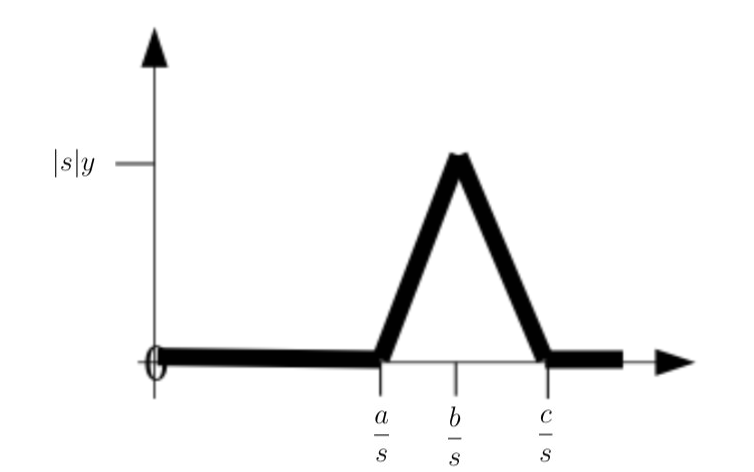
\includegraphics[]{figure1.png}
	    
	\section*{Exercise 7.2}
	\textbf{a.} Linearity: $\widehat{x(\omega) + y(\omega)} = \hat{x}(\omega) + \hat{y}(\omega)$
	\begin{alignat*}{2}
		\widehat{x(\omega) + y(\omega)} &= \sum_{n \in \inte} (x(n) + y(n)) \cdot \een\\
		&= \sum_{n \in \inte} x(n) \cdot \een + y(n) \cdot \een\\
		&= \sum_{n \in \inte} x(n) \cdot \een + \sum_{n \in \inte} y(n) \cdot \een
		&= \hat{x}(\omega) + \hat{y}(\omega)
	\end{alignat*}
	Linearity: $\widehat{\lambda x(\omega)} = \lambda\hat{x}(\omega)$
	\begin{alignat*}{2}
		\widehat{\lambda x(\omega)} &= \sum_{n \in \inte} \lambda x(n) \cdot \een\\
		&= \lambda \sum_{n \in \inte} x(n) \cdot \een
		&= \lambda\hat{x}(\omega)
	\end{alignat*}


	\textbf{b.} Time Shift: $\hat{x_k}(\omega) = \eek \hat{x}(\omega)$, $n' = n-k, n= n'+k$
	\begin{alignat*}{2}
		\hat{x_k}(\omega) &= \sum_{n \in \inte} x_k(n) \cdot \een\\
		&= \sum_{n \in \inte} x(n-k) \cdot \een\\
		&= \sum_{n' \in \inte} x(n') \cdot e^{-2\pi i \omega (n'+k)}\\
		&= \sum_{n' \in \inte} x(n') \cdot e^{-2\pi i \omega n'} \cdot e^{-2\pi i \omega k}\\
		&= e^{-2\pi i \omega k} \sum_{n' \in \inte} x(n') \cdot e^{-2\pi i \omega n'} 
		&= \eek \hat{x}(\omega)
	\end{alignat*}


	\textbf{c.} Frequency Shift: $\widehat{x^{\omega_0}}(\omega) = \hat{x}(\omega + \omega_0)$
	\begin{alignat*}{2}
		\widehat{x^{\omega_0}}(\omega) &= \sum_{n \in \inte} x^{\omega_0}(n) \cdot \een\\
		&= \sum_{n \in \inte} e^{-2\pi i \omega_0 n}x(n) \cdot \een\\
		&= \sum_{n \in \inte} x(n) \cdot e^{-2\pi i \omega_0 n - 2\pi i \omega n}\\
		&= \sum_{n \in \inte} x(n) \cdot e^{-2\pi i n (\omega + \omega_0)}
		&= \hat{x}(\omega + \omega_0)
	\end{alignat*}
	
	
	\textbf{d.} Frequency Reversal: $y(n) = \overline{x(n)} \implies \hat{y}(\omega) = \overline{\hat{x}(-\omega)}$
	\begin{alignat*}{2}
		\hat{y}(\omega) &= \sum_{n \in \inte} y(n) \cdot \een\\
		&= \sum_{n \in \inte} \overline{x(n)} \cdot \een\\
		&= \overline{\sum_{n \in \inte} x(n) \cdot e^{2\pi i \omega n}}\\
		&= \overline{\sum_{n \in \inte} x(n) \cdot e^{-2\pi i (-\omega) n}}
		&= \overline{\hat{x}(-\omega)}
	\end{alignat*}
	because $\overline{\hat{x}(\omega)} = \sum_{n \in \inte} \overline{x(n)} \cdot e^{2\pi i \omega n}$.
	
	
	\textbf{e.} Time Reversal: $ \forall n, \text{ if } y(n) = x(-n) \text{ then } \hat{y}(\omega) = \hat{x}(-\omega), m = -n$
	\begin{alignat*}{2}
		\hat{y}(\omega) &= \sum_{n \in \inte} y(n) \cdot \een\\
		&= \sum_{n \in \inte} x(-n) \cdot \een\\
		&= \sum_{n \in \inte} x(m) \cdot e^{2\pi i \omega m}\\
		&= \sum_{n \in \inte} x(m) \cdot e^{-2\pi i (-\omega) m}
		&= \hat{x}(-\omega)
	\end{alignat*}
	\section*{Exercise 7.3}
	\textbf{a-c.} The solutions can be found inside the \texttt{code} folder.
\end{document}
